%https://tikz.net/dynamics_spring/
\documentclass[border=3pt,tikz]{standalone}
\usetikzlibrary{snakes}
\usetikzlibrary{patterns}

\begin{document}
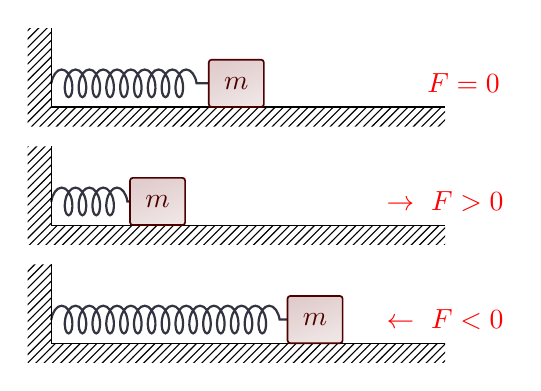
\begin{tikzpicture}[
    ground/.style={fill,pattern=north east lines,draw=none,minimum width=0.3,minimum height=0.6},
    spring/.style={line width=0.8,blue!7!black!80,snake=coil,segment amplitude=5,segment length=5,line cap=round},
    mass/.style={line width=0.6,red!30!black,fill=red!40!black!10,rounded corners=1,
    top color=red!40!black!20,bottom color=red!40!black!10,shading angle=20}
    ]
    \def\H{1}    % wall height
    \def\T{0.3}  % wall thickness
    \def\W{5.0}  % ground length
    \def\D{0.25} % ground depth
    \def\h{0.6}  % mass height
    \def\w{0.7}  % mass width
    \def\x{1.6}  % mass x position
    % \def\x{1.6}  % mass x position

    \foreach \y/\x in {0/2.0,1.5/1.0,3/3.0} {
        \begin{scope}[shift={(0,-\y)}]
            \draw[spring] (0,\h/2) --++ (\x,0);
            \draw[ground] (0,0) |-++ (-\T,\H) |-++ (\T+\W,-\H-\D) -- (\W,0) -- cycle;
            \draw (0,\H) -- (0,0) -- (\W,0);
            \draw[mass] (\x,0) rectangle++ (\w,\h) node[midway] {$m$};
        \end{scope}
    }
    \node [red] at (\W,\h/2) {$\phantom{\rightarrow~}F=0$};
    \node [red] at (\W,\h/2-1.5) {$\rightarrow~F>0$};
    \node [red] at (\W,\h/2-3) {$\leftarrow~F<0$};
\end{tikzpicture}
\end{document}
